\chapter{Analisi dei dati e  risultati di ricerca} %\label{1cap:spinta_laterale}
% [titolo ridotto se non ci dovesse stare] {titolo completo}
%
     \section{Data Cleaning}
    
    Come osservato precedentemente, il survey Prolific, ha raccolto un totale di 203 risposte totali. Prima di partire con l'effettiva analisi dei dati però, si è reso necessario validare la consistenza e l'integrità delle risposte ricevute. Inizialmente 19 sottomissioni sono state considerate inattendibili e quindi rimosse dal dateset di partenza per i seguenti motivi:
    
    \begin{itemize}
        \item 17 sono state considerate inattendibili a causa di risposte errate alle domande poste come attenction check di verifica, quindi successivamente eliminate dal dataset originale.
        \item 2 risposte sono state eliminate, osservando inconguenze con l'identificativo Prolific immesso.
    \end{itemize}
     
    Delle 184 sottomissioni restanti, c'è inoltre da considerare che 68 partecipanti hanno dichiarato di non aver alcuna esperienza con lo sviluppo di moduli AI-intensive, quindi sono stati direttamente condotti alla sezione di chiusura del Survey elettronico, anche se mantenute nel dataset di partenza, tali risposte (per strutturazione intrinseca del survey) non possedevano informazioni utili per rispondere i quesiti di ricerca, ma data la presenza di quesiti aperti e contatti utili, esse sono state trasferite in un dataset secondario da utilizzare per successive fasi di approfondimento. I restanti 116 partecipanti all'indagine hanno invece dichiarato di avere effettivamente esperienza con lo sviluppo di soluzioni AI-Intensive, quindi le risposte relative sono state ritenute utili al fine di elaborare i risultati dello studio in risposta agli obiettivi di ricerca prefissati precedentemente.\\  
    
    
    Da notare inoltre come 18 partecipanti dei 116 restanti (con esperienza nello sviluppo di soluzioni AI-Intensive), abbiano lasciato a disposizione un loro contatto email per eventuali interviste future, o per ottenere nuovi aggiornamenti circa l'elaborazione dei risultati.  
    
    \section{Pre-processing}
    Prima di procedere con il vero e proprio lavoro di analisi, è stato necessario applicare alcune piccole trasformazioni ai dati grezzi, e consequenzialmente prima di illustrare il lavoro di analisi, si riportano riferimenti alle trasformazioni applicate al dataset, utili a interpretare i risultati ottenuti in maniera più agevole.
    
    \subsection{Mapping tra quesiti del survey e obiettivi di ricerca}
    
    Al fine di comprendere meglio quali quesiti, posti ai partecipanti all'indagine empirica, forniscano dati utili a rispondere ad uno specifico quesito di ricerca, il dataset di risposte iniziale, è stato diviso in 5 dataset più piccoli, ciascuno corrispondente ad uno specifico sub-goal di ricerca formalizzato precedentemente. La successiva tabella 5.1 riassume i dettagli dell'attività di mapping.
    
    \begin{longtable}{| p{.90\textwidth} |} 
        
        \hline
        \rowcolor{Gray}
        \textbf{\textit{{RQ1.1}}}:  Quali sono i migliori approcci e definizioni per trattare la fairness in un contesto lavorativo?\\
        
        \hline 
         Secondo te, quali dei seguenti aspetti rappresentano la definizione generica di fairness fornita in precedenza?
         \\ \hline
        Considerando la tua esperienza lavorativa, quanto i seguenti (approcci) sono trattati?
        \\ \hline
        Generalmente utilizzi altri approcci per lavorare con il concetto di Software Fairness?
        \\ \hline
        
        \rowcolor{Gray}
        \textbf{\textit{{RQ1.2}}}:  Com'è generalmente composto un team lavorativo per lo sviluppo di moduli ML-Intensive Fair Critical?\\
        
        \hline 
         Considerando i seguenti ruoli (professionali), chi ha impatto sulle scelte inerenti la software fairness?
       
        \\ \hline
        \rowcolor{Gray}
        \textbf{\textit{{RQ1.3}}}:  Quanto il concetto di software fairness è importante se paragonato ad altri aspetti non funzionali?\\
        
        \hline 
         Considerando i seguenti aspetti (funzionali e non funzionali) dello sviluppo software, quanto li ritieni importanti se comparati alla fairness?
         
        \\ \hline
        \rowcolor{Gray}
        \textbf{\textit{{RQ1.4}}}:  In quali fasi di una tipica pipeline di Machine Learning è importante adottare strategie per garantire alti livelli di fairness?\\
        
        \hline 
         Considerando una generica pipeline di machine learning (come la seguente - figura 4.1), quanto consideri l’equità come un aspetto rilevante per ciascuna delle seguenti fasi nel tuo contesto lavorativo?
         
         \\ \hline
        Quali tool utilizzi (se previsti) per trattare la fairness in una pipeline di machine learning ?
        
        \\ \hline
        \rowcolor{Gray}
        \textbf{\textit{{RQ1.5}}}:  Quanto le compagnie di sviluppo ML-Intensive, sono mature nel trattare il concetto di fairness come un requisito non funzionale?\\
        
        \hline 
        In quale dei seguenti livelli di maturità, classificheresti il tuo ambiente lavorativo circa il trattamento della fairness?
        \\ \hline
        \caption{Survey Question \& Research goal mapping} % needs to go inside longtable environment
    \label{tab:myfirstlongtable}
    \end{longtable}
    
    \subsection{Abbreviazioni e trasformazioni di scala}
    
    Considerando che molti concetti formalizzati sul questionario, sono stati espressi in forma discorsiva per garantirne una maggiore comprensione ai partecipanti all'indagine, si è reso necessario convertirli prima della fase di aggregazione dei dati, in valori facilmente compatibili agli strumenti automatici di analisi utilizzati. I quesiti specifici, per cui si è resa necessaria questa attività, sono state quindi formalizzate due tipologie di scale, una quantitativa o riassuntiva (composta da alias per il concetto espresso in forma discorsiva) e una qualitativa (contenente le vere e proprie opzioni di risposta alla domanda di riferimento).\\
    
    Le successive tabelle riassumono quindi per intero le trasformazioni di scala applicate.\\\\
    
    
    \subsubsection{Definizioni di fairness e abbreviazioni}
    
    \begin{center}
		\hspace*{-5mm}\begin{tikzpicture}
			\node [mybox] (box){%
				\begin{minipage}{.70\textwidth}
					\centering
					
                    	\textit{RQ1.1 - Quesito: Secondo te, quali dei seguenti aspetti rappresentano la definizione generica di fairness fornita in precedenza?}
				
				\end{minipage}
			};
		\end{tikzpicture}%
	\end{center}
	
     \begin{longtable}{| p{.30\textwidth} | p{.55\textwidth} |} 
      
      \hline\textbf{\textit{Valore Riassuntivo}} & \textbf{\textit{Valore qualitativo (risposte)}}
       
        
        \\ \hline
        \rowcolor{Gray}
        Definizioni Probabilistiche        
        
        &   Treating similar individuals in a way that they are equally likely to receive a specific outcome

        
        \\ \hline


        Definizioni basate su similarità matematica      
        
        &  Do not favor certain subjects over others on the basis of sensitive attributes, e.g., race, gender, etc.




        \\ \hline
        \rowcolor{Gray}
        Definizioni basate su casual reasoning       
        
        &  Taking decisions by protecting individuals and groups from mistreatments

        
        \\ \hline
        \caption{Mapping tra le tipologie di definizione di fairness e la loro forma discorsiva} % needs to go inside longtable environment
        \label{tab:myfirstlongtable}
    \end{longtable}
    
    
     \subsubsection{Approcci al trattamento della fairness e abbreviazioni}
    
    \begin{center}
		\hspace*{-5mm}\begin{tikzpicture}
			\node [mybox] (box){%
				\begin{minipage}{.70\textwidth}
					\centering
					
                    	\textit{RQ1.1 - Quesito: Considerando la tua esperienza lavorativa, quanto i seguenti (approcci) sono trattati?}
				
				\end{minipage}
			};
		\end{tikzpicture}%
	\end{center}
	
     \begin{longtable}{| p{.30\textwidth} | p{.55\textwidth} |} 
      
      \hline\textbf{\textit{Valore Riassuntivo}} & \textbf{\textit{Valore qualitativo (risposte)}}
       
        
        \\ \hline
        \rowcolor{Gray}
        Approccio 1       
        
        &   We focus on guaranteeing high probability to obtain ethically correct outcomes regardless of sensitive features


        
        \\ \hline


        Approccio 2      
        
        &  We focus on guaranteeing that machine learning predictions are not going to discriminate by sensitive features





        \\ \hline
        \rowcolor{Gray}
        Approccio 3      
        
        &  We model the relation between attributes and outcomes, verifying that the outcome does not depend on sensitive attributes


        
        \\ \hline
        \caption{Mapping tra le tipologie di approcci alla  fairness e la loro forma discorsiva} % needs to go inside longtable environment
        \label{tab:myfirstlongtable}
    \end{longtable}
    
    \subsubsection{Cambiamenti di scala per l'applicabilità di definizioni e approcci alla fairness}
    
    \begin{center}
		\hspace*{-5mm}\begin{tikzpicture}
			\node [mybox] (box){%
				\begin{minipage}{.70\textwidth}
					\centering
					
                    	\textit{RQ1.1 - Quesito: Secondo te, quali dei seguenti aspetti rappresentano la definizione generica di fairness fornita in precedenza?}
				
				\end{minipage}
			};
		\end{tikzpicture}%
	\end{center}
	
    \begin{center}
		\hspace*{-5mm}\begin{tikzpicture}
			\node [mybox] (box){%
				\begin{minipage}{.70\textwidth}
					\centering
					
                    	\textit{RQ1.1 - Quesito: Considerando la tua esperienza lavorativa, quanto i seguenti (approcci) sono trattati?}
				
				\end{minipage}
			};
		\end{tikzpicture}%
	\end{center}
	
     \begin{longtable}{| p{.25\textwidth} | p{.35\textwidth} |} 
      
      \hline\textbf{\textit{Scala quantitativa}} & \textbf{\textit{Valore qualitativo (risposte)}}
       
        
        \\ \hline
        \rowcolor{Gray}
        1       
        
        &  Not at all


        
        \\ \hline


        2     
        
        & Slightly



        \\ \hline
        \rowcolor{Gray}
        3     
        
        &  Neutral

        
        \\ \hline


        4    
        
        & To a great extent



        \\ \hline
        
        \rowcolor{Gray}
        5
        
        &  Extremely

        \\ \hline
        \caption{Scale qualitativa e quantitativa per la valutazione di definizioni e approcci} % needs to go inside longtable environment
        \label{tab:myfirstlongtable}
    \end{longtable}
\newpage
\subsubsection{Cambiamenti di scala circa l'impatto professionale nel trattamento della fairness}
    
    \begin{center}
		\hspace*{-5mm}\begin{tikzpicture}
			\node [mybox] (box){%
				\begin{minipage}{.70\textwidth}
					\centering
					
                    	\textit{RQ1.2 - Quesito: Considerando i seguenti ruoli (professionali), chi ha impatto sulle scelte inerenti la software fairness?}
				
				\end{minipage}
			};
		\end{tikzpicture}%
	\end{center}
	
     \begin{longtable}{| p{.25\textwidth} | p{.35\textwidth} |} 
      
      \hline\textbf{\textit{Scala quantitativa}} & \textbf{\textit{Valore qualitativo (risposte)}}
       
        
        \\ \hline
        \rowcolor{Gray}
        1       
        
        &  Very low impact



        
        \\ \hline


        2     
        
        & Below average impact




        \\ \hline
        \rowcolor{Gray}
        3     
        
        &  Average impact


        
        \\ \hline


        4    
        
        & Above average impact




        \\ \hline
        
        \rowcolor{Gray}
        5
        
        &  Very high impact


        \\ \hline
        \caption{Scale qualitativa e quantitativa per la valutazione dell'impatto professionale} % needs to go inside longtable environment
        \label{tab:myfirstlongtable}
    \end{longtable}
    
\subsubsection{Cambiamenti di scala circa la valutazione di importanza della fairness rispetto altri NFR}
    
    \begin{center}
		\hspace*{-5mm}\begin{tikzpicture}
			\node [mybox] (box){%
				\begin{minipage}{.70\textwidth}
					\centering
					
                    	\textit{RQ1.3 - Quesito: Considerando i seguenti aspetti (funzionali e non funzionali) dello sviluppo software, quanto li ritieni importanti se comparati alla fairness?}
				
				\end{minipage}
			};
		\end{tikzpicture}%
	\end{center}
	
     \begin{longtable}{| p{.25\textwidth} | p{.40\textwidth} |} 
      
      \hline\textbf{\textit{Scala quantitativa}} & \textbf{\textit{Valore qualitativo (risposte)}}
       
        
        \\ \hline
        \rowcolor{Gray}
        -2    
        
        &  Less important than fairness


        \\ \hline


        -1     
        
        & A bit less important than fairness

        \\ \hline
        \rowcolor{Gray}
        0    
        
        &  Neutral

        \\ \hline


        1    
        
        & A bit more important than fairness





        \\ \hline
        
        \rowcolor{Gray}
        2
        
        &  More important than fairness



        \\ \hline
        \caption{Scale qualitativa e quantitativa per la valutazione dei fairness trade-offs} % needs to go inside longtable environment
        \label{tab:myfirstlongtable}
    \end{longtable}
    
    
    
    \subsubsection{Cambiamenti di scala circa l'utilità di applicazione di strategie Fair-Oriented in una pipeline ML}
    
    \begin{center}
		\hspace*{-5mm}\begin{tikzpicture}
			\node [mybox] (box){%
				\begin{minipage}{.70\textwidth}
					\centering
					
                    	\textit{RQ1.4 - Considerando una generica pipeline di machine learning (come la seguente - figura 4.1), quanto consideri l’equità come un aspetto rilevante per ciascuna delle seguenti fasi nel tuo contesto lavorativo?}
				
				\end{minipage}
			};
		\end{tikzpicture}%
	\end{center}
	
     \begin{longtable}{| p{.25\textwidth} | p{.40\textwidth} |} 
      
      \hline\textbf{\textit{Scala quantitativa}} & \textbf{\textit{Valore qualitativo (risposte)}}
       
        
        \\ \hline
        \rowcolor{Gray}
        1    
        
        &  Not at all

        \\ \hline


        2    
        
        & Slightly


        \\ \hline
        \rowcolor{Gray}
        3   
        
        &  Neutral

        \\ \hline


        4   
        
        & Very


        \\ \hline
        
        \rowcolor{Gray}
        5
        
        &  Extremelly


        \\ \hline
        \caption{Scale qualitativa e quantitativa per l'impatto di fairness su una Pipeline di Machine Learning} % needs to go inside longtable environment
        \label{tab:myfirstlongtable}
    \end{longtable}
    
    \newpage
    \subsubsection{Livelli di maturità aziendale e spiegazine relativa}
    
    \begin{center}
		\hspace*{-5mm}\begin{tikzpicture}
			\node [mybox] (box){%
				\begin{minipage}{.70\textwidth}
					\centering
					
                    	\textit{RQ1.5 - In quale dei seguenti livelli di maturità, classificheresti il tuo ambiente lavorativo circa il trattamento della fairness?}
				
				\end{minipage}
			};
		\end{tikzpicture}%
	\end{center}
	
     \begin{longtable}{| p{.20\textwidth} | p{.60\textwidth} |} 
      
      \hline\textbf{\textit{Livello}} & \textbf{\textit{Spiegazione}}
       
        
        \\ \hline
        \rowcolor{Gray}
        Livello 0    
        
        &  We do not treat software fairness

        \\ \hline


       Livello 1    
        
        & We occasionally treat software fairness,  but related processes are disorganized and even chaotic



        \\ \hline
        \rowcolor{Gray}
        Livello 2   
        
        &  We regularly treat fairness and related processes are established, defined and documented


        \\ \hline


        Livello 3   
        
        & We regularly treat fairness and it develops its own standard fairness management processes



        \\ \hline
        
        \rowcolor{Gray}
        Livello 4
        
        &  We regularly treat fairness and it monitors and controls its own fairness related processes through data collection and analysis


        \\ \hline


        Livello 5  
        
        & We regularly treat fairness and fairness related processes are constantly improved through monitoring feedback


        \\ \hline
        \caption{Scale qualitativa e quantitativa per l'impatto di fairness su una Pipeline di Machine Learning} % needs to go inside longtable environment
        \label{tab:myfirstlongtable}
    \end{longtable}
    
    \newpage
    \section{Analisi dei dati}
    Una volta realizzate le dovute trasformazioni di scala e la sistematizzazione dei concetti, il campione empirico, risulta quindi pronto per essere effettivamente analizzato. Ovviamente per la fase di analisi, è stato necessario selezionare un opportuno tool, che automatizzasse l'aggregazione statistica de dati e la formulazione di grafici descrittivi, tra le varie alternative disponibili, a tale scopo è stato selezionato il linguaggio statistico R e la libreria ggplot2 per la formulazione di grafici descrittivi.
    
    \subsection{Composizione del campione}
    
    Prima di cominciare effettivamente con l'analizzare i risultati specifici di ogni sub-goal di ricerca, è opportuno effettuare qualche considerazione sul campione di 116 individui considerati validi dopo la fase di data cleaning. \\

    
    \begin{figure}[h]
        \centering
        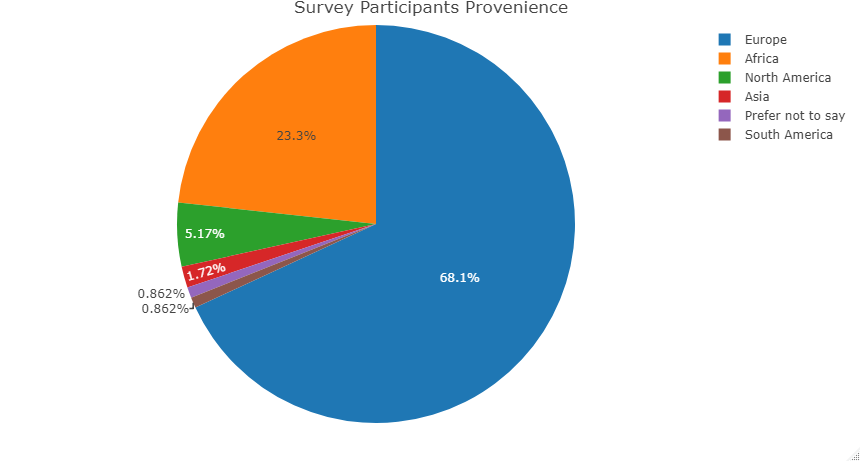
\includegraphics[width=1\textwidth]{figure/Analisi/Background/Survey_Partecipants_Provenience.png}
        \caption{Distribuzione continentale del campione di analisi}
    \end{figure}
    
    Come osservabile dalla figura 5.1, il campione di analisi, è principalmente concentrato tra Europa e Africa, ciò significa appunto che le deduzioni successive, questo dettaglio non è trascurabile, dato che la generalizzabilità dei risultati, potrebbe essere messa in discussione, per aree geografiche rappresentate in maniera minore. Ad ogni modo, questo prima considerazione, è senz'altro da attribuire al fatto che Prolific è essenzialmente una piattaforma di origine britannica, quindi maggiormente pubblicizzata in Europa. Nel dettaglio, 79 partecipanti hanno dichiarato di provenire dall'europa, 27 dall'africa, 6 dal nord america, 2 dall'asia, 1 dal sud america, mentre 1 ha preferito non dichiarare la sua provenienza.
    
    \begin{figure}[h]
        \centering
        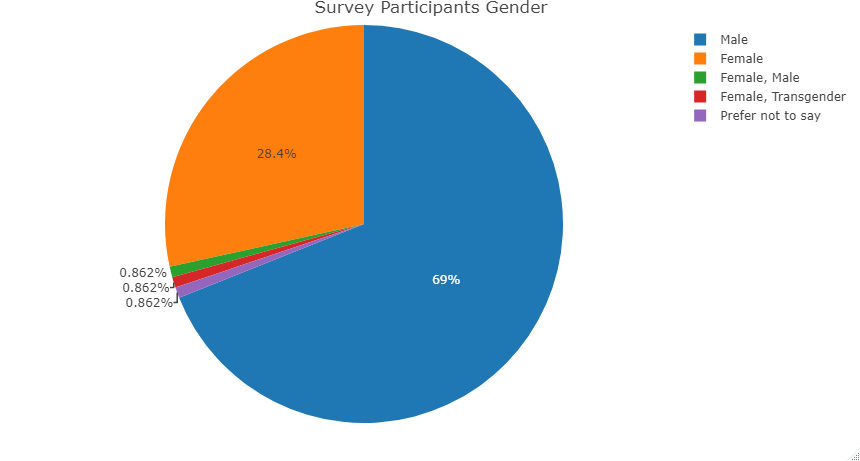
\includegraphics[width=1\textwidth]{figure/Analisi/Background/Survey_Partecipants_Gender.png}
        \caption{Distribuzione di gender nel campione di analisi}
    \end{figure}
    
    Analogamente alla provenienza, con la figura 5.2 è possibile effettuare qualche considerazione analoga, con l'identificazione di gender dei partecipanti. la presenza di tale quesito è stato ampiamente discussa in fase di progettazione del questionario, dato che essa è spesso un informazione da ritenere altamente discriminatoria se non non richiesta nel modo giusto, a tale scopo, è stata introdotta l'opzione di controllo Prefer Not To Say, che tuttavia è stata selezionata solo da un partecipante su 116. 80 invece si identificano nel gender maschile, 33 in in quello femminile, 1 in entrambi i precedenti, 1 come Transgender e donna contemporaneamente.\\
    
    \begin{figure}[h!]
        \centering
        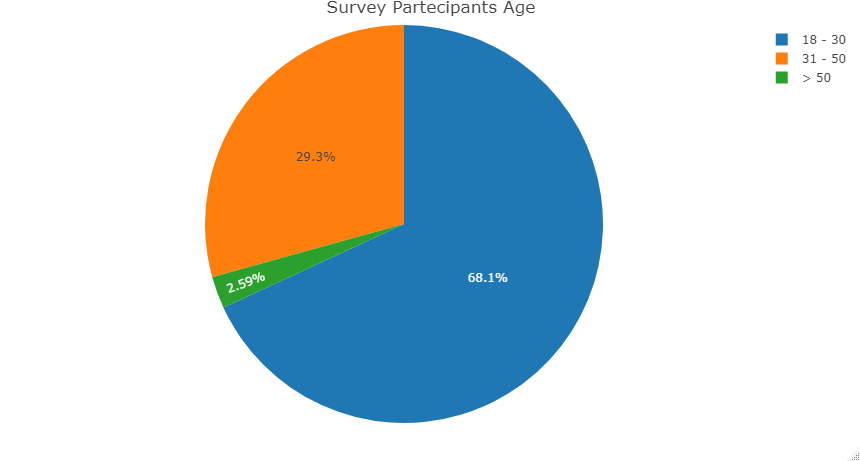
\includegraphics[width=1\textwidth]{figure/Analisi/Background/Survey_Partecipants_Age.png}
        \caption{Distribuzione dell'età nel campione di analisi}
    \end{figure}
    
   Considerando invece la figura 5.3 è possibile notare, come la maggioranza del campione, si concentri maggiormente tra i 18 e i 30 anni, più nello specifico 79 partecipanti si colloca in questo range, 34 invece sono i partecipanti appartenenti alla fascia di età tra i 31 e i 50 anni, portando quindi anche maggiore maturità professionale al campione, mentre infine 3 partecipanti dichiarano di possedere più di 50 anni.
   
   \begin{figure}[h!]
        \centering
        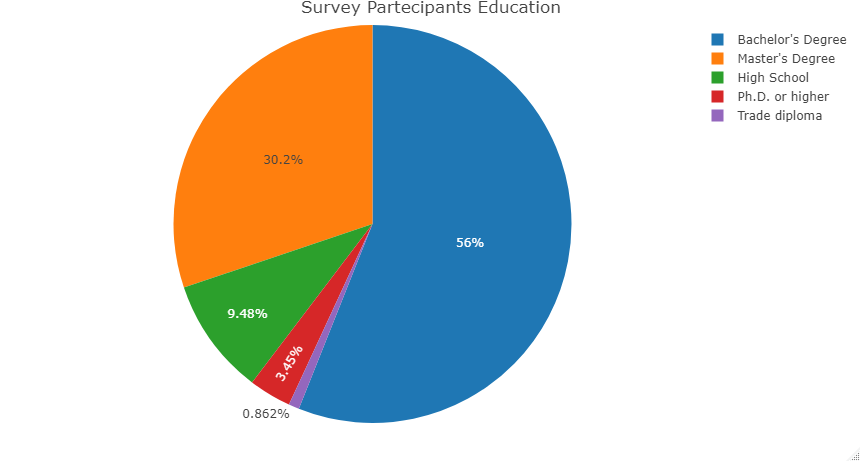
\includegraphics[width=1\textwidth]{figure/Analisi/Background/Survey_Partecipants_Education.png}
        \caption{Distribuzione del livello di studi nel campione di analisi}
    \end{figure}
   Fin dall'inizio della fase di progettazione del Survey, al fine dell'attendibilità delle informazioni ricevute è stata considerato come fattore di rilevante importanza il livello di studio medio dei partecipanti, preferendo in particolare un alto livello di studio (laurea triennale e superiori), dalla figura 5.4 è osservabile come tale tendenza sia rispettata da quasi tutti i partecipanti all'indagine, nel dettaglio su 116 partecipanti totali, 65 dichiarano di possedere almeno un titolo di studi triennale, 35 invece dichiarano di aver conseguito un titolo magistrale, 4 risultano aver completato anche il dottorato di ricerca, mentre i restati 12 si dividono in 11 con un diploma di istruzione superiore e un singolo con diploma professionale.\\
   
   Continuando poi con la posizione e il ruolo professionale dei partecipanti, è possibile notare come effettivamente, il campione degli intervistati sia abbastanza variegato e corrispondente ai requisiti di appartenenza precedentemente fissati. 
   
    \begin{figure}[h!]
        \centering
        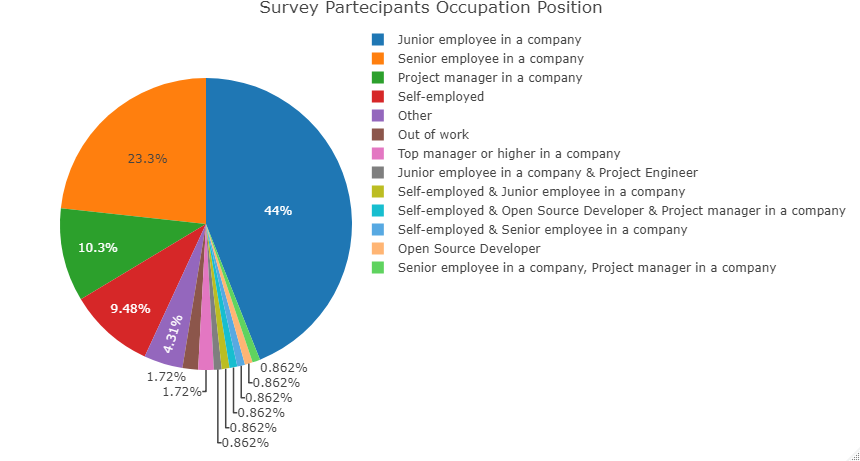
\includegraphics[width=1\textwidth]{figure/Analisi/Background/Survey_Partecipants_Occupation_Position.png}
        \caption{Livello di occupazione professionale dei partecipanti all'analisi}
    \end{figure}
    
    In particolare, come osserva la figura 5.5, la maggioranza dei partecipanti ricopre un ruolo attivo in una compagnia, nel dettaglio è possibile dividere questa fetta in 51 impiegati aziendali junior, 27 impiegati aziendali Senior, e 12 Project Manager e 2 come Top-Manager  in azienda. Tra i restanti, 11 si dichiarano come lavoratori autonomi. Tra i restanti, ci sono figure professionali singole, che dichiarano di ricoprire più di una posizione professionale contemporaneamente o altri ruoli quali sviluppatore open source, infine risultano esserci 5 partecipanti che dichiarano di avere altra posizione altro rispetto a quelle specificate, mentre solo 2 risultano disoccupati al momento della sottomissione.  
    
      \begin{figure}[h!]
        \centering
        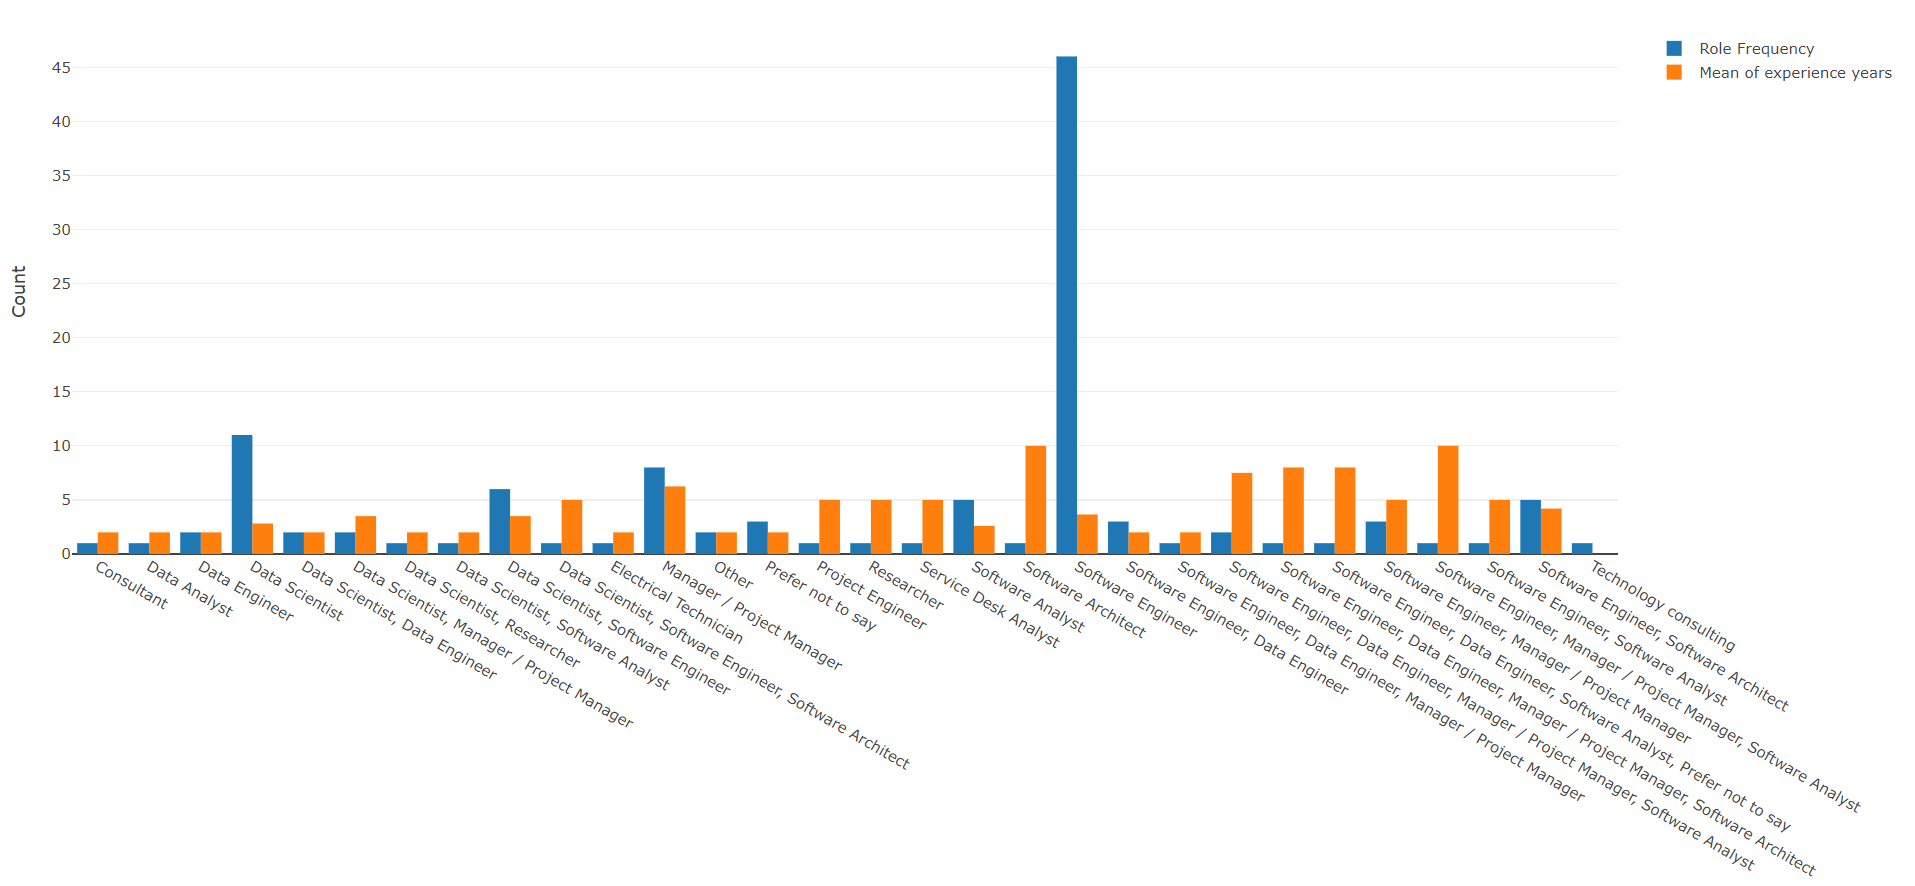
\includegraphics[width=0.8\textwidth]{figure/Analisi/Background/Survey_Partecipants_Roles.png}
        
        \caption{Ruoli professionali dei partecipanti all'analisi}
    \end{figure}
    
    Dando invece uno sguardo ai ruoli professionali, è possibile osservare come circa la metà o poco più dei partecipanti, abbia affinità con l'ingegneria del software, l'ingegneria dei dati, e il management, leggermente meno ampia è la presenza di ruoli affini a posizioni quali Data Science o altri ruoli professionali, mentre in media. Mentre è di rilievo considerare che tutti i partecipanti hanno in media dai 2 ai 10 anni di esperienza nel ruolo indicato. Da un punto di vista empirico, l'eterogeneità del campione è senz'altro molto positiva dato che sia per via dei differenti ruoli, che per i variegati livelli di occupazione, è possibile dare più valenza statistica alle successive informazioni estratte dai dati grezzi.
    
    \subsection{Fairness in pratica, come rispondere al quesito generale?}
    
    
    \begin{center}
		\hspace*{-5mm}\begin{tikzpicture}
			\node [mybox] (box){%
				\begin{minipage}{.70\textwidth}
					\centering
					
                    	\textit{RQ1: In che modo il concetto di Software Fairness è attualmente percepito nell'ambiente lavorativo ML-Intensive?}
				
				\end{minipage}
			};
		\end{tikzpicture}%
	\end{center}
	
	Come più volte osservato più volte, cercar di raccogliere dati utili a rispondere in maniera formale a questo unico macro-quesito, può essere qualcosa di generalmente complesso e forse anche riduttivo da proporre per un concetto così variegato come quello di Software Fairness, sicuramente considerando l'andamento generale dell'analisi dei dati, così come viene riportato nei successivi paragrafi, è senz'altro facile capire che, come stabilito dalla ricerca Fairness, è un concetto estremamente variabile ed in evoluzione, quindi così come per la fase di progettazione, anche quella di analisi risulta essere più assimilabile se scomposta in sotto-punti speculari ai sub-goal di ricerca definiti. 
    
    \subsection{Applicabilità di definizioni e approcci per fairness}
    
    \begin{center}
			\hspace*{-5mm}\begin{tikzpicture}
			\node [mybox] (box){%
				\begin{minipage}{.70\textwidth}
					\centering
					\textit{RQ1.1 - Quali sono i migliori approcci e definizioni per trattare la fairness in un contesto lavorativo?}
				\end{minipage}
			};
		\end{tikzpicture}%
	\end{center}
    
     \begin{figure}[h!]
        \centering
        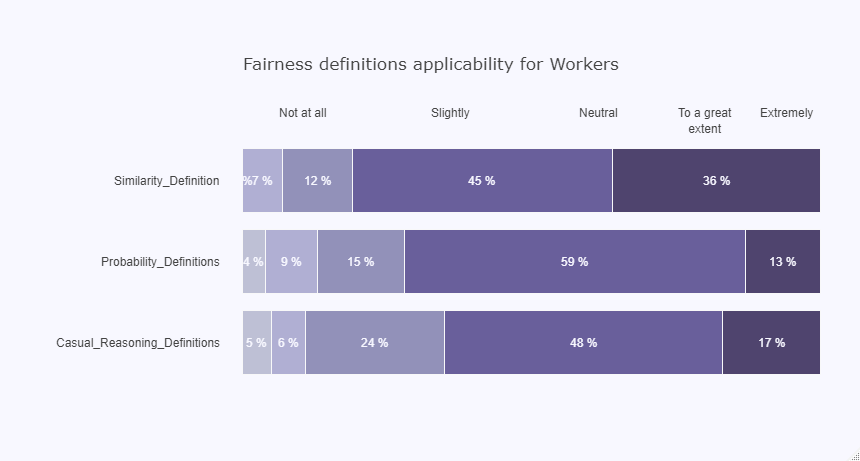
\includegraphics[width=1\textwidth]{figure/Analisi/RQ1/Hist_Fairness_Deginitions_Applicability.png}
        \caption{Definizioni di fairness in ambito lavorativo}
    \end{figure}
    
    Data l'ampia variabilità del concetto, non è corretto porre un quesito di ricerca che voglia definire univocamente il concetto o la definizione \emph{aziendale} di software fairness. Da un punto di vista analitico, la figura 5.7, dimostra infatti come per gli esperti, tutte le tipologie di definizioni e metriche teoriche, possono essere ampiamente applicate in casi reali di sviluppo, per tutte e tre i gruppi di definizione, i livelli 4 e 5 delle scale di applicabilità superano il 50\% dei consensi, a seconda dei contesti di applicazioni e dei requisiti specifici del modulo ML. Da un'analisi più attenta, però si osserva come ad avere maggior margine di applicazione (anche se non di misura), risultino essere gli approcci alla misurazione basati su \textbf{statistica matematica} e secondariamente quelli basati su \textbf{probabilità}.  
    
      \begin{figure}[h!]
        \centering
        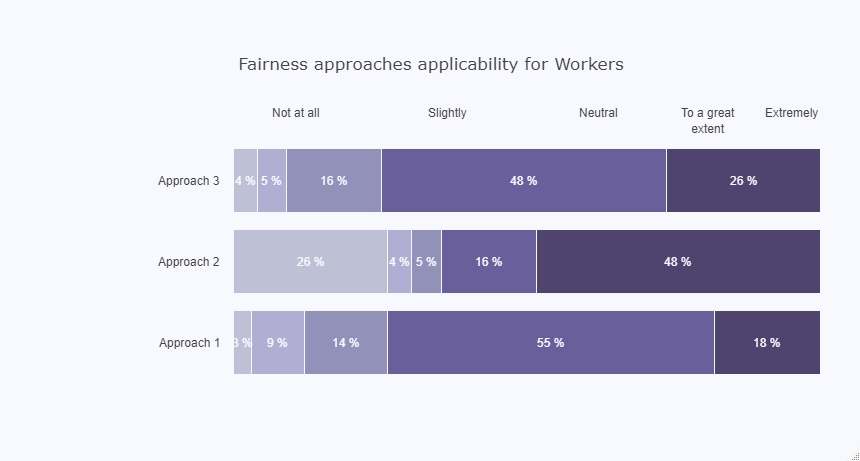
\includegraphics[width=1\textwidth]{figure/Analisi/RQ1/Hist_Fairness_Approaches_Applicability.png}
        \caption{Approcci al concetto di fairness in ambito lavorativo}
    \end{figure}
    
    Passando invece all'analisi degli approcci, si osserva facilmente come in azienda prevalga facilmente l'idea che \textbf{i livelli alti di Software Fairness}, vadano ricercati cercando di \textbf{ridurre le dipendenze tra gli attributi sensibili e i risultati predetti} (approccio 1), e quasi specularmente nel \textbf{cercare di ridurre le dipendenze tra attributi sensibili e risultati}. Meno percepito come applicabile, risulta essere invece il secondo approccio proposto, ovvero concentrarsi nel garantire che il learner non effettui valutazioni discriminatorie sulla base di feature sensibili. Ciò è probabilmente da attribuire, alla complessità di questa seconda opzione proposta, non facilmente intuibile e difficilmente analizzabile rispetto le altre due.\\
    
    Ovviamente anche in azienda, il concetto di fairness non si limita a quanto espresso in teoria, esso può essere visto a vari livelli di dettaglio, e soprattutto in riferimento al dominio di utilizzo. A dimostrazione di ciò, risultano interessanti molte risposte ottenute al terzo quesito (risposta aperta breve) progettato per questo primo sub-goal di ricerca, ovvero: Generalmente utilizzi altri approcci per lavorare con il concetto di Software Fairness?
	
	Segue un breve report di alcune delle considerazioni più interessanti:
	
	\begin{itemize}
	    \item Approcci Domain Specific - Provare a rendere i risultati disponibili a persone con disabilità, quindi in sostanza, renderli equi per tutti; 
	    \item Metodologie Empiriche - Condurre survey e ottenere in cosiderazioni opinioni diverse;
	    \item Ottimizzazione nella gestione dei dati - Ottenere dei dati di training sensibili abbastanza affinchè i risultati siano il meno possibile discriminanti;
	    \item Analisi di correlazione - Analizzare la correlazione forte-debole tra risultati e features;
	\end{itemize}
    
    \subsection{Impatto professionale per il trattamento della fairness}
	\begin{center}
		\hspace*{-5mm}\begin{tikzpicture}
			\node [mybox] (box){%
				\begin{minipage}{.70\textwidth}
					\centering
					\textit{RQ1.2 - Come è composto generalmente un team lavorativo per lo sviluppo di moduli ML-Intensive Fair Critical?}
				\end{minipage}
			};
		\end{tikzpicture}%
	\end{center}
	
	  \begin{figure}[h!]
        \centering
        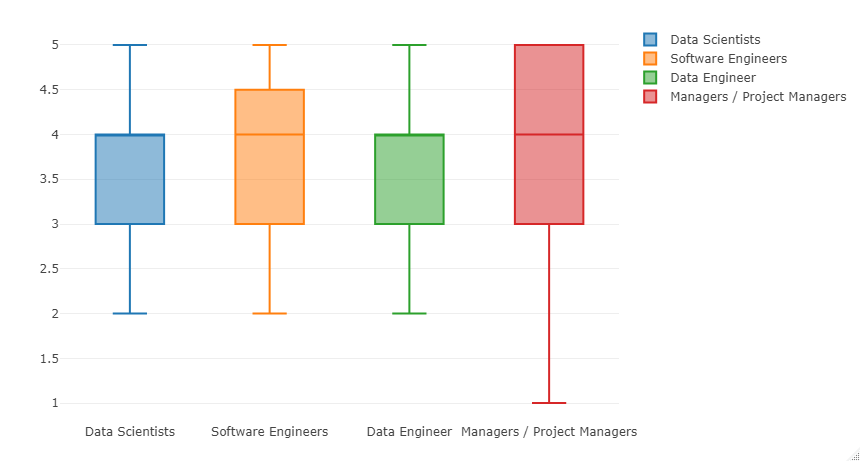
\includegraphics[width=1\textwidth]{figure/Analisi/RQ2/RoleImpactBoxPlot1.png}
        \caption{Ruoli professionali durante lo sviluppo Fair Oriented 1/2}
    \end{figure}
    
     \begin{figure}[h!]
        \centering
        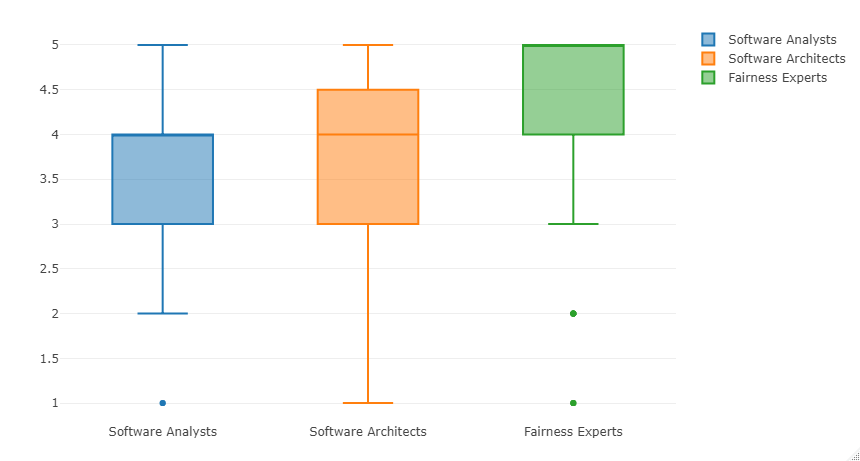
\includegraphics[width=1\textwidth]{figure/Analisi/RQ2/RoleImpactBoxPlot2.png}
        \caption{Ruoli professionali durante lo sviluppo Fair Oriented 2/2}
    \end{figure}
	 
	 
	 Osservando le figure 5.9 e 5.10, è facilmente intuibile, come \textbf{tutti i ruoli professionali} proposti,vengano considerati cruciali durante lo sviluppo di una soluzione fair critical, infatti il valore mediano per ogni figura professionale si attesta almeno a 4 (secondo valore di rilevanza nella scala precedentemente illustrata). Volendo entrare più nel dettaglio, è possibile osservare come \textbf{manager} ed \textbf{esperti specifici}, siano figure estremamente di rilievo e utili nella gestione degli aspetti di equità di un modulo di Machine Learning. Risultano molto simili sono invece attribuibili a figure come Data Scientist, Data Engineer e Ingegneri del software, a dimostrazione del fatto che, anche in un contesto reale, mantenere alta la sinergia tra queste due branche dello sviluppo ML-Intensive sia cruciale soprattutto in contesti molto specifici come quello della fairness. Da notare come ci sia una leggera presenza di outliers per ruoli come Analisti ed Esperti di fairness (basso impatto in controtendenza con il resto del campione), ma ciò è da considerare come fattore eccezionale, dato che tali figure possono essere comunque molto specifiche e magari non presenti in ogni ambiente lavorativo dei partecipanti all'indagine.
    \subsection{Confronto tra fairness con altre caratteristiche qualitative non funzionali}
    
    \begin{center}
		\hspace*{-5mm}\begin{tikzpicture}
			\node [mybox] (box){%
				\begin{minipage}{.70\textwidth}
					\centering
					\textit{RQ1.3 - Quanto il concetto di software fairness è importante se paragonato ad altri aspetti non funzionali?}
				\end{minipage}
			};
		\end{tikzpicture}%
	\end{center}
	Come visto più volte, analizzare la fairness, come un vero e proprio attributo non funzionale di prima classe sia la chiave di lettura al fine di eliminare fault etici latenti in un modulo di machine learning \cite{brun2018software}. Ovviamente chiedere richiedere tale sforzo ai professionisti è un qualcosa di molto ostico soprattutto mettendo a paragone Fairness, con requisiti molto più standardizzati, quali accuracy o sicurezza. Ma analizzando i risultati, è possibile provare ad osservare qualche deduzione interessante.\\
	
	N.B. nei successivi diagrammi, sono state rappresentate le densità delle singole risposte dei partecipanti, in blu si può notare la fetta di persone che considera uno specifico requisito altamente meno importante rispetto a Fairness (-2 della scala quantitativa) , in verde è racchiusa la parte di campione che considera fairness leggermente più importate rispetto all'altro requisito analizzato dal diagramma (-1 della scala quantitativa), in giallo quella che considera fairness rilevante quanto il requisito confrontato (0 nella scala quantitativa), in arancione quella fetta di campione che considera il requisito in analisi lievemente più importante rispetto a fairness (+1), mentre in rosso gli individui che considerano il requisito specifico altamente più importante di fairness (+2).
	\begin{figure}[h!]
        \centering
        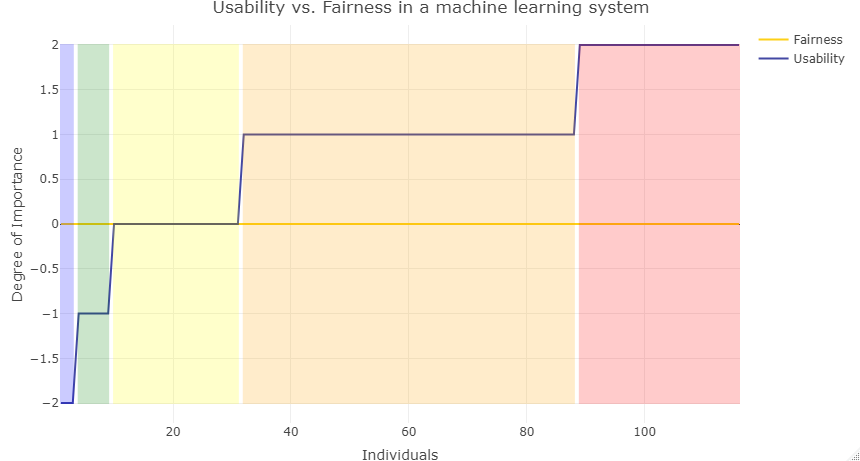
\includegraphics[width=1\textwidth]{figure/Analisi/RQ3/1.Usability_vs_Fairness.png}
        \caption{Fairness vs Usabilità}
    \end{figure}
    
    \begin{figure}[h!]
        \centering
        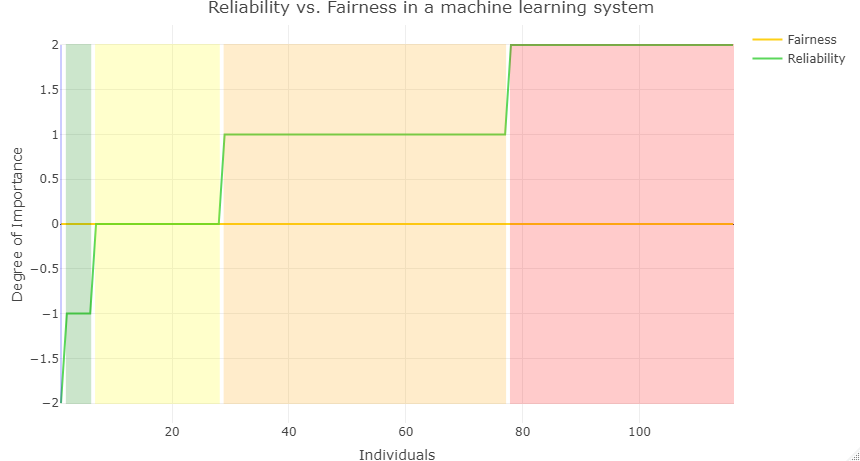
\includegraphics[width=1\textwidth]{figure/Analisi/RQ3/2.Reliability_vs_Fairness.png}
        \caption{Fairness vs Affidabilità}
    \end{figure}
    
    \begin{figure}[h!]
        \centering
        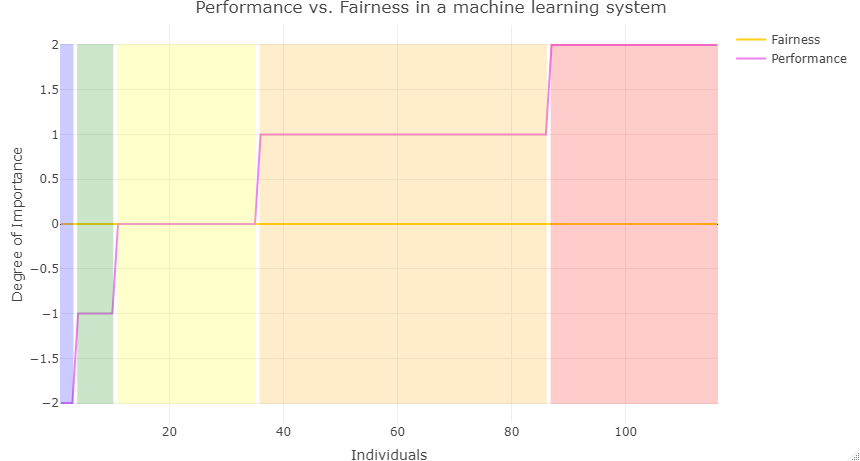
\includegraphics[width=1\textwidth]{figure/Analisi/RQ3/3.Performance vs. Fairness.png}
        \caption{Fairness vs Performances}
    \end{figure}
    
    
    \begin{figure}[h!]
        \centering
        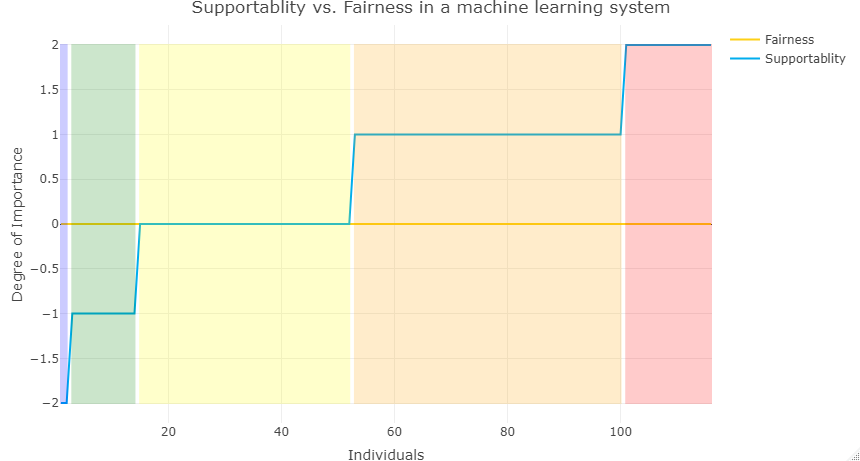
\includegraphics[width=1\textwidth]{figure/Analisi/RQ3/4.Supportablity vs. Fairness.png}
        \caption{Fairness vs Supportabilità}
    \end{figure}
    
    
    Come osservabile dalle figure 5.11 alla 5.14, aspetti non funzionali standard, del noto modello furps+ (usabilità, affidabilità, performance e supportabilità), sono aspetti che per la maggior parte del campione, risultano essere di misura più rilevanti di fairness, in particolare si osserva che per aspetti particolarmente critici per i moduli di intelligenza artificiale, quali \textbf{affidabilità e performances}, la fetta di persone che li considera \textbf{estremamente più importanti}, sale anche \textbf{sopra le 25/30 unità}, per diminuire leggermente negli altri aspetti riportati. È però da tener conto come quasi tutti gli aspetti del modello iniziale analizzato (Furps+), come fairness, siano altamente variabili a seconda delle necessità del tool specifico, infatti, osservando come la maggior parte dei partecipanti consideri \textbf{usabilità e supportabilità} leggermente più impattanti nello sviluppo ml-intensive, rispetto fairness, si può sicuramente lasciare margine di confronto tra questi attributi e fairness a seconda delle specifiche esigenze.
    \begin{figure}[h!]
        \centering
        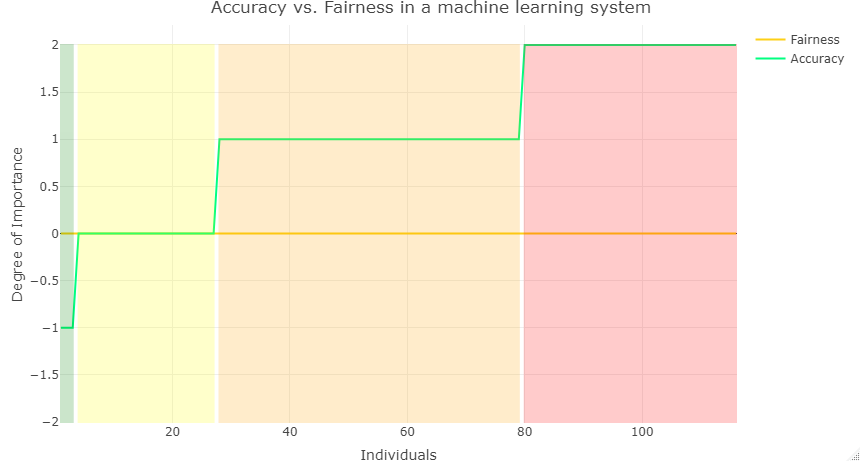
\includegraphics[width=1\textwidth]{figure/Analisi/RQ3/5.Accuracy vs. Fairness.png}
        \caption{Fairness vs Accuracy}
    \end{figure}
    
     \begin{figure}[h!]
        \centering
        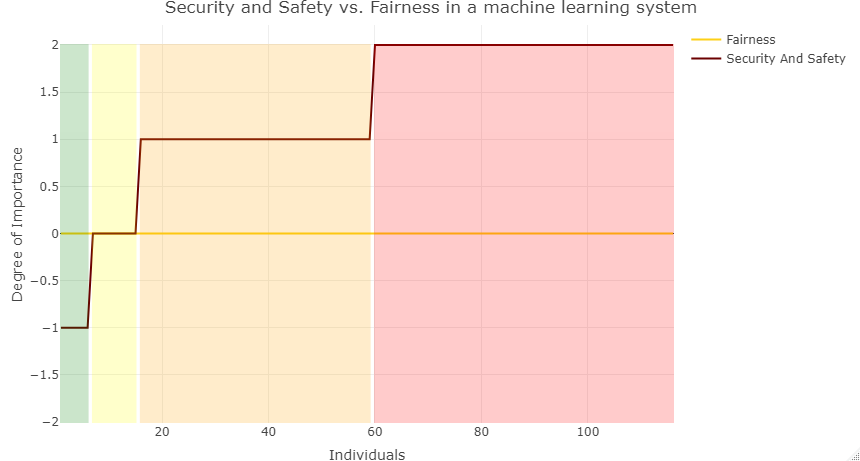
\includegraphics[width=1\textwidth]{figure/Analisi/RQ3/6.Security and Safety.png}
        \caption{Fairness vs Sicurezza}
    \end{figure}
    
    Il discorso cambia di misura per aspetti già più specifici per un canonico modello di machine learning, infatti sia per accuracy che sicurezza, nessuno dei partecipanti ha ritenuto opportuno indicarli come ampiamente meno importanti rispetto alla fairness, inoltre per questi due aspetti anche la finestra di voto che va da -1 a 0, risulta essere molto ristretta. Sia \textbf{l'accuracy che la Sicurezza, sono da considerare da lievemente ad estremamente più rilevanti} rispetto a fairness sulla base del campione. Ciò molto probabilmente è dovuto al fatto che chi lavora quotidianamente con questi sistemi, in maniera quasi automatica si troverà a lavorare a problematiche di accuracy o sicurezza del modello, cosa non sempre così semplice (almeno allo stato attuale delle cose) per fairness. 
    \begin{figure}[h!]
        \centering
        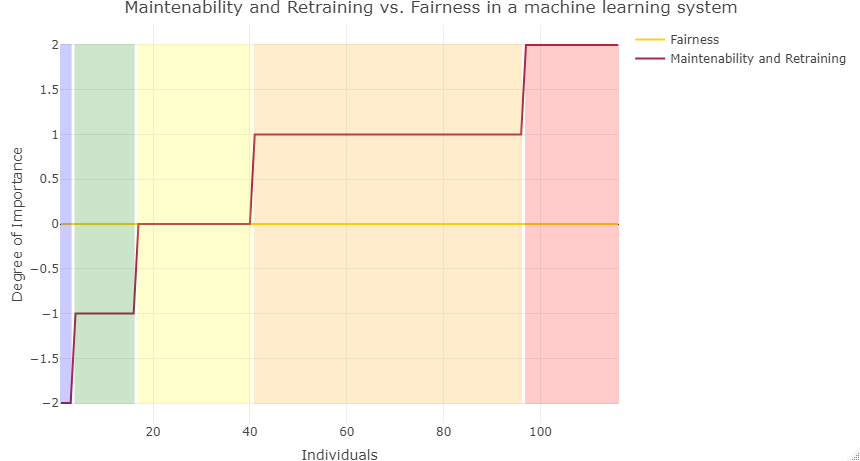
\includegraphics[width=1\textwidth]{figure/Analisi/RQ3/7.Maintenability and Retraining.png}
        \caption{Fairness vs Manutenibilità e Retraining}
    \end{figure}
    
    \begin{figure}[h!]
        \centering
        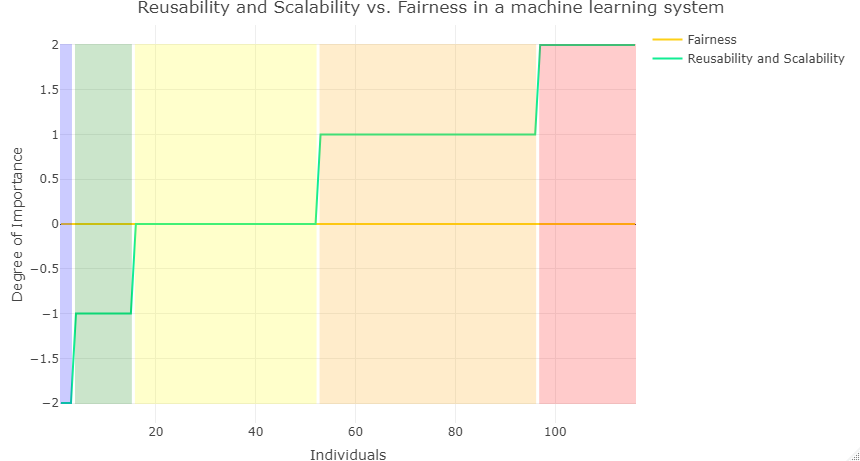
\includegraphics[width=1\textwidth]{figure/Analisi/RQ3/8.Reusability and Scalability.png}
        \caption{Fairness vs Riusabilità e Scalabilità}
    \end{figure}
    
    In maniera più semplificata (aggregando i concetti), è stato chiesto ai partecipanti di provare a fornire un parere similare alle altre specifiche non funzionali quali manutenibilità \& retraining - figura 5.17 (in ottica evolutiva di un generico tool ML-Intensive) e scalabilità \& riusabilità - figura 5.18. Per questa tipologia di requisiti, i report grafici, possono facilmente far dedurre considerazioni similari rispetto al modello Furps+, ma probabilmente per arrivare ad osservazioni più precise, si dovrebbe analizzare separatamente i singoli dati (scelta non adottata per evitare di rendere troppo complesso il quesito ai partecipanti).\\\\
    
    In generale, le problematiche discriminatorie ed il concetto di software fairness, sono probabilmente concetti molto distanti dagli aspetti di qualità, già ampiamente studiati e sistematizzati. Allo stato della pratica, il generico lavoratore, sia esso data scientist, ingegnere del software, manager o quant'altro, difficilmente darà  più rilevanza in termini assoluti a fairness rispetto ad altre prerogative non funzionali (a maggior ragione per aspetti critici, quali accuracy, performance o sicurezza), e le cause possono essere molteplici, ad esempio:
    
    \begin{itemize}
        \item Probabilmente la rilevanza del concetto di fairness aumenterà mano a mano che la società percepirà le problematiche connesse come un problema prioritario, quindi tali confronti dovranno essere ripetuti in futuro;
        \item Fairness probabilmente necessita di essere analizzata in maniera diversa rispetto gli aspetti non funzionali standard, probabilmente in ragione alla specificità del dominio;

    \end{itemize}
    
    \subsection{Fairness come aspetto intrinseco di una pipeline ML}

    	\begin{center}
    	\hspace*{-5mm}\begin{tikzpicture}
    		\node [mybox] (box){%
    			\begin{minipage}{.70\textwidth}
    				\centering
    				\textit{RQ1.4 - In quali fasi di una tipica pipeline di Machine Learning è importante adottare strategie per garantire alti livelli di fairness?}
    			\end{minipage}
    		};
    	\end{tikzpicture}%
    \end{center}
    
     \begin{figure}[h!]
        \centering
        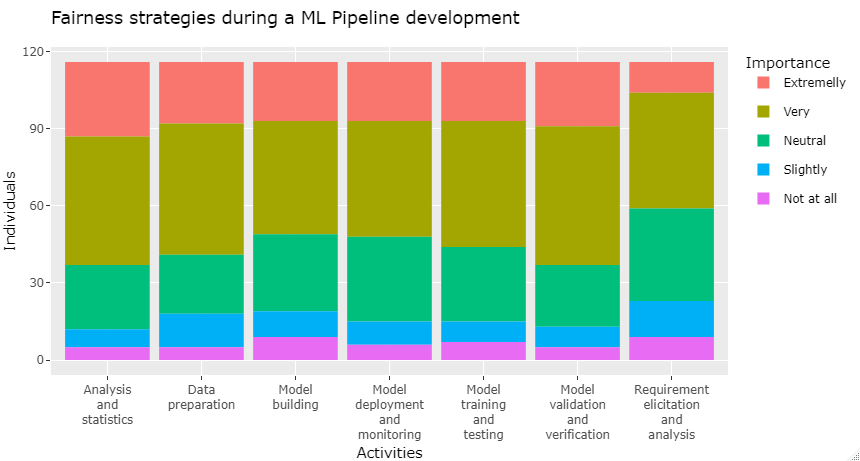
\includegraphics[width=1\textwidth]{figure/Analisi/RQ4/Fairness strategies during a ML Pipeline development.png}
        \caption{Applicabilità di strategie di Fairness improoving in una Pipeline di Machine learining}
    \end{figure}
    Come già osservato in fase di progettazione, questo specifico sub goal, mira a valutare l'utilità di adottare strategie di fairness level improoving in ogni fase di una generica pipeline di machine learning. Dai dati e dal report grafico di figura 5.19, è  evidenziabile, come la \textbf{fairness di un sistema di machine learning è un aspetto di rilevanza in ogni fase di una generica pipeline}, ma da un occhiata più specifica, è facile dedurne come essa stessa può essere un aspetto qualitativo che migliora mano a mano che il sistema evolve sia dopo la fase di building, \textbf{dato che la fase di verifica e validazione viene considerata una delle più valide} per attestare il livello di fairness del sistema, \textbf{seguita dalla fase di analisi e statistica} (successiva al deploy del modello), e di conseguenza dalla \textbf{fase di preparazione dei dati}, che ovviamente va raffinata ad ogni ciclo di sviluppo di una tipica pipeline ML. Ciò significa che la pratica lavorativa, secondo i dati raccolti, probabilmente suggerisce che attualmente la Fairness è un aspetto di un modello di machine learning che va di pari passo con la sua evoluzione, ed è probabilmente lì che è necessario investire con soluzioni specifiche.
    
    \begin{figure}[h!]
        \centering
        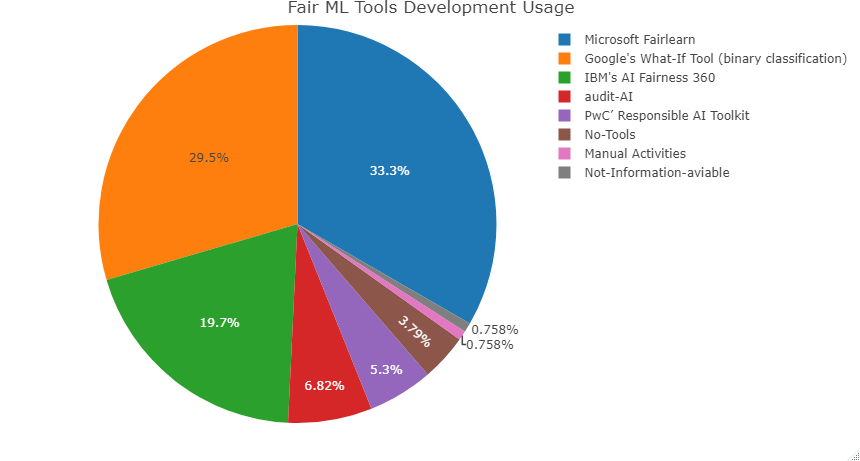
\includegraphics[width=1\textwidth]{figure/Analisi/RQ4/Fair ML Tools Development Usage.png}
        \caption{Utilizzo di tool noti per il Fair ML Development}
    \end{figure}
    
    Per fornire altri dettagli circa l'utilizzo di approcci e strumenti utili al trattamento di fairness come aspetto integrante del ciclo di sviluppo di un modulo ml, si osserva (figura 5.20) letteralmente pochi partecipanti all'indagine abbiano fatto dichiarato di non fare uso di tool specifici per il fairness improoving. la maggior parte di essi invece dichiara di aver utilizzato almeno una volta un tool proprietario tra i noti Microsoft Fairlearn, Google's-What-IF o IBM's AI Fairness 360. Ciò è sicuramente un buon segnale, dato che le aziende evidentemente, sono molto propense ad adottare strategie specifiche per progettare soluzioni ML Fair su larga scala.
    \subsection{Fairness e maturità aziendale}
    
    \begin{center}
    	\hspace*{-5mm}\begin{tikzpicture}
    		\node [mybox] (box){%
    			\begin{minipage}{.70\textwidth}
    				\centering
    				\textit{RQ1.5 - Quanto le compagnie di sviluppo ML-Intensive, sono mature nel trattare il concetto di fairness come un requisito non funzionale?}
    			\end{minipage}
    		};
    	\end{tikzpicture}%
    \end{center}
    
    Ultimo punto conclusivo della panoramica analitica sullo stato della pratica lavorativa, è appunto cercare di capire se e come le aziende dei partecipanti all'indagine definiscono la problematica di fairness durante un generico progetto di sviluppo ML-Intensive e soprattutto quanto sono mature le politiche aziendali a riguardo. 
    
    \begin{figure}[h!]
        \centering
        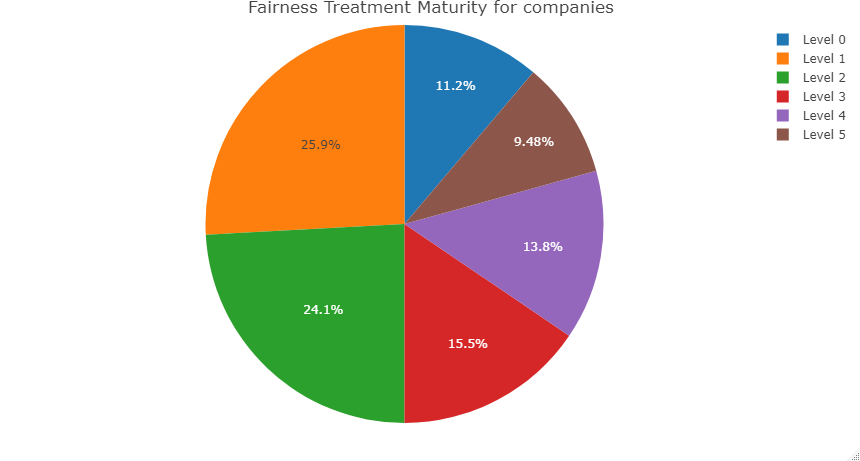
\includegraphics[width=1\textwidth]{figure/Analisi/RQ5/Fairness Treatment Maturity for companies.png}
        \caption{Risultati analitici del Fair Capability Maturity Model}
    \end{figure}
    
    Come risporta la figura 5.21, è facile fornire una risposta preliminare a questo questo di ricerca, il contesto attuale, provando a generalizzare quanto osservabile sulla base del campione, è costituito da circa un \textbf{50\% delle aziende che praticano sviluppo di soluzioni ML-Intensive}, che tratta fairness ai \textbf{livelli 1 e 2}, ovvero, secondo la scala prefissata, trattano le problematiche connesse alla fairness in maniera sporadica o abitudinaria, ma senza l'utilizzo di standard specifici. Interessante anche come dell'altra metà dei partecipanti, soltanto \textbf{l'11,2\% dichiari che la sua azienda non tratti affatto fairness}, infatti \textbf{la fetta restante di partecipanti colloca la propria azienda ai livelli 3, 4 e 5}, quindi dal trattare Fairness in maniera abitudinaria con specifici standard di sviluppo, fino all'applicazione di tecniche di process improoving sugli specifici processi aziendali. 
    
     \begin{figure}[h!]
        \centering
        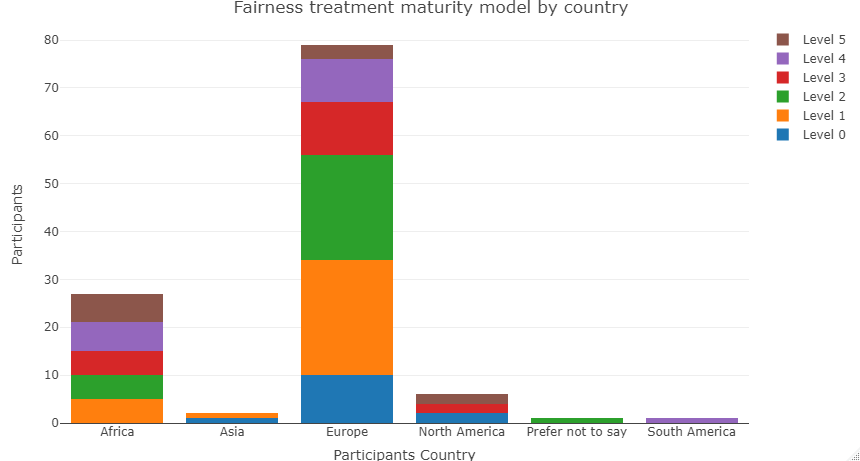
\includegraphics[width=1\textwidth]{figure/Analisi/RQ5/Fairness treatment maturity model by country.png}
        \caption{Risultati analitici del Fair Capability Maturity Model per continente}
    \end{figure}
    
    Spostando l'analisi su un ottica più mirata, come quella continentale, si nota ancora meglio come ad esempio in Europa (la maggioranza del campione) le aziende pratichino processi atti alla gestione della fairness. Ciò è senz'altro un fattore ampiamente positivo, dato che è facilmente osservabile come le aziende, ad esempio su scala europea, siano disposte a migliorare e ad applicare processi ingegneristici nell'ambito ml intensive, di pari passo all'evoluzione metodologica della ricerca e degli investimenti pubblici \cite{ritson201317}.
    \section{Minacce alla validità}

\newpage
